% ----------------------------------------------------------------------------
% Author: Rayla Kurosaki
% GitHub: https://github.com/rkp1503
% ----------------------------------------------------------------------------
\section{Figures}\label{sec:figures}
\begin{figure}
    \centering
    \subfloat[Stability of the interior equilibrium.]{%
    \resizebox*{7cm}{!}{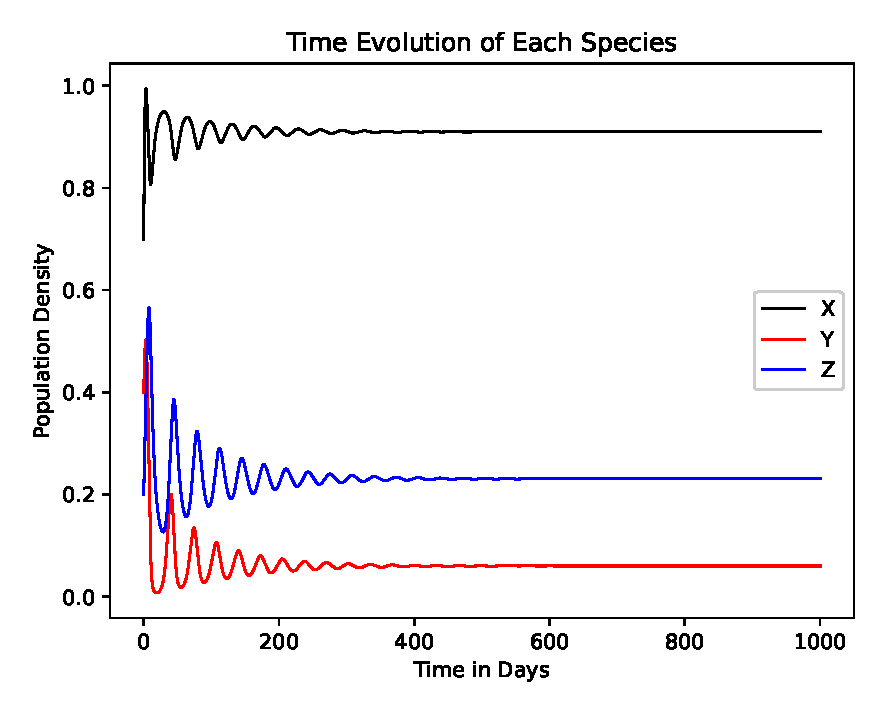
\includegraphics{equilibrium-interior-time-evolution.eps}\label{fig:time-evolution}}}\hspace{5pt}
    \subfloat[3D phase portrait.]{%
    \resizebox*{7cm}{!}{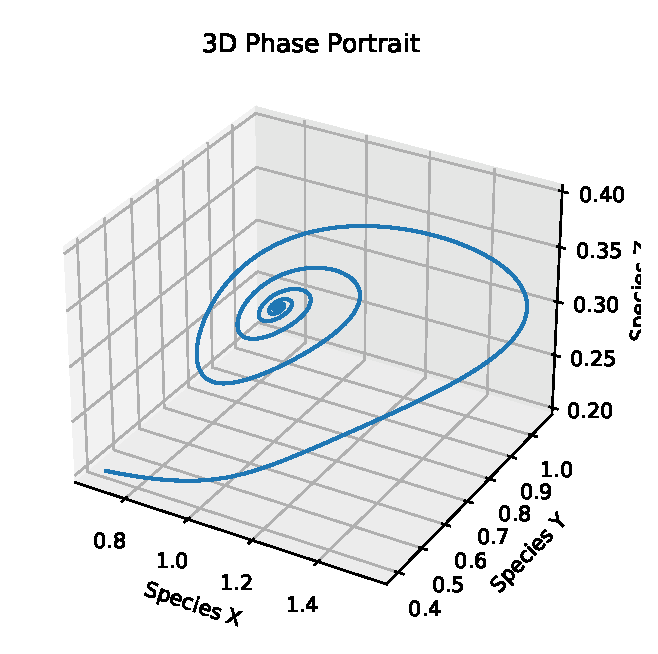
\includegraphics{equilibrium-interior-pp-xyz.eps}\label{fig:phase-plane-3d}}}\hspace{5pt}
    \subfloat[$xy$-phase plane.]{%
    \resizebox*{7cm}{!}{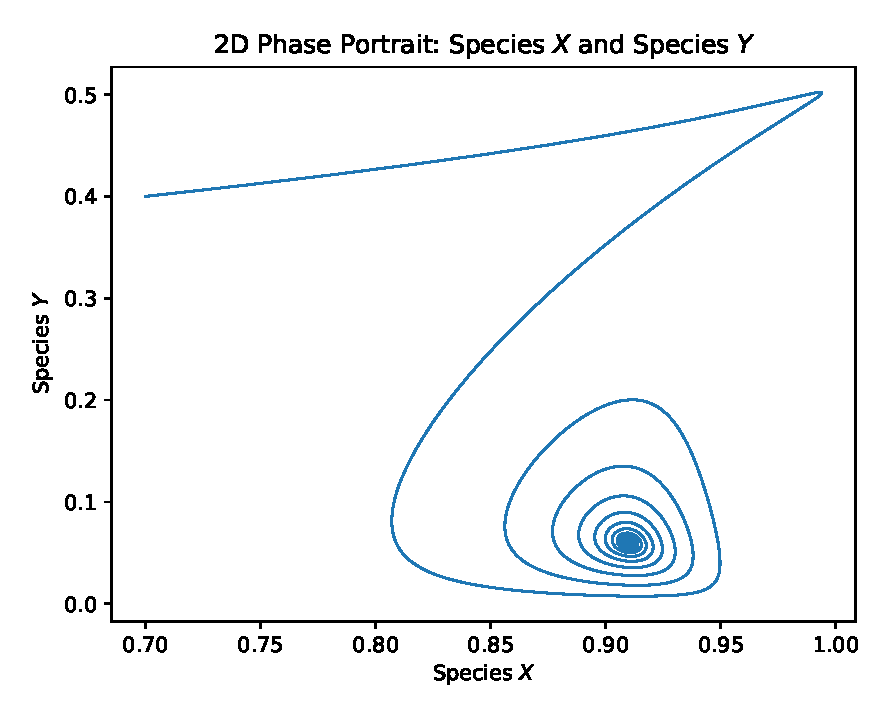
\includegraphics{equilibrium-interior-pp-xy.eps}\label{fig:phase-plane-xy}}}\hspace{5pt}
    \subfloat[$xz$-phase plane.]{%
    \resizebox*{7cm}{!}{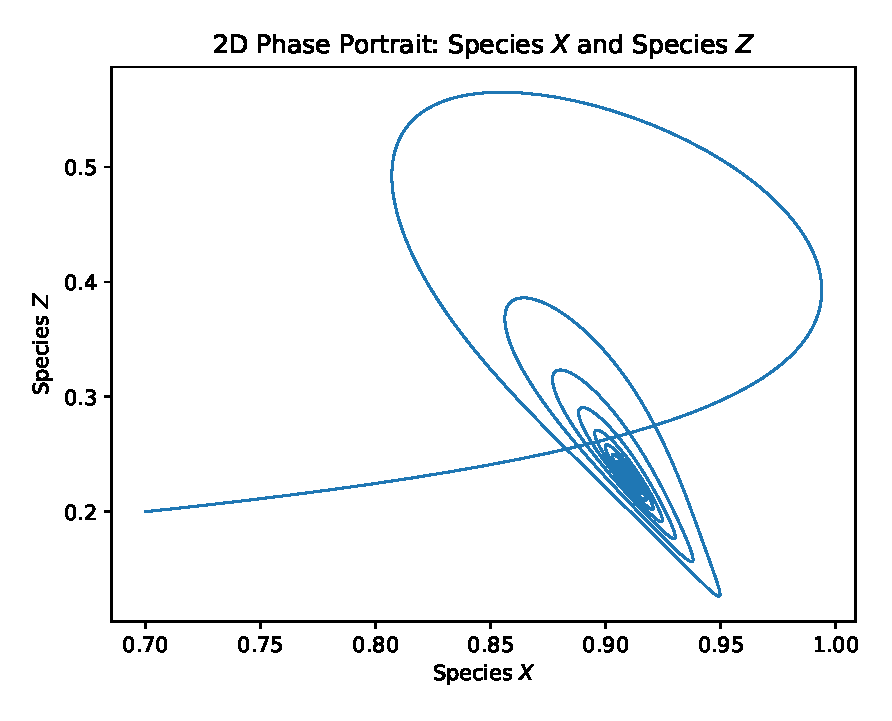
\includegraphics{equilibrium-interior-pp-xz.eps}\label{fig:phase-plane-xz}}}\hspace{5pt}
    \subfloat[$yz$-phase plane.]{%
    \resizebox*{7cm}{!}{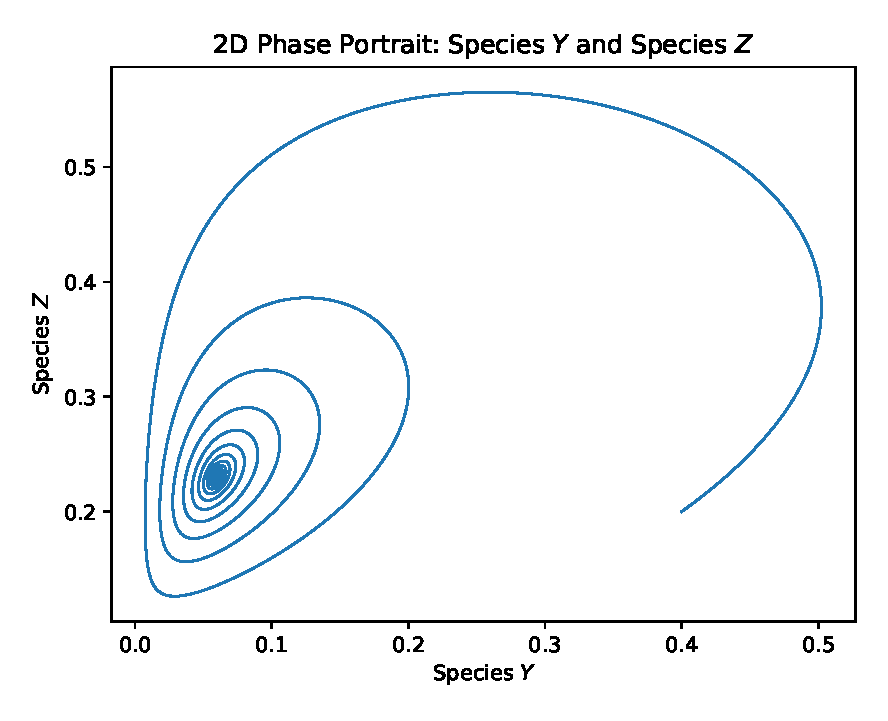
\includegraphics{equilibrium-interior-pp-yz.eps}\label{fig:phase-plane-yz}}}
    \caption{Different types of plots to show the behavior of \myref[Model]{model:rayla-ephraim} under the set of \myref[parameters]{params:interior-a}.}
    \label{fig:nontrivial-equilibria-plots}
\end{figure}

\begin{figure}[!htb]
    \centering
    \subfloat[Time Evolution of each species where $r_{yx}=0.5$]{%
    \resizebox*{5cm}{!}{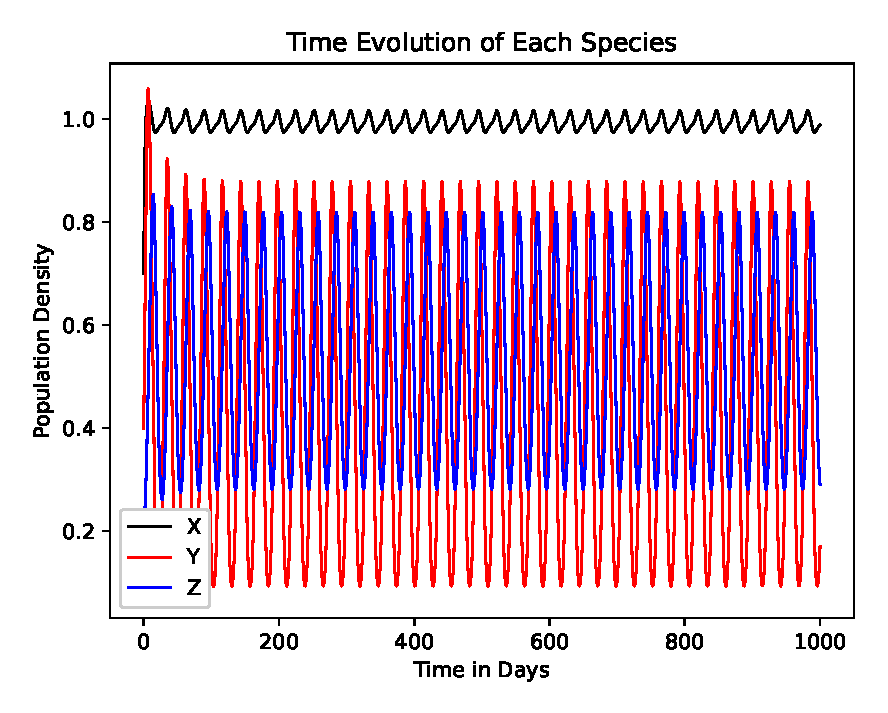
\includegraphics{equilibrium-interior-bifurcation-r_yx.eps}\label{fig:bifurcation-r_yx-xyz}}}\hspace{5pt}
    \subfloat[Bifurcation diagram of Species $X$]{%
    \resizebox*{5cm}{!}{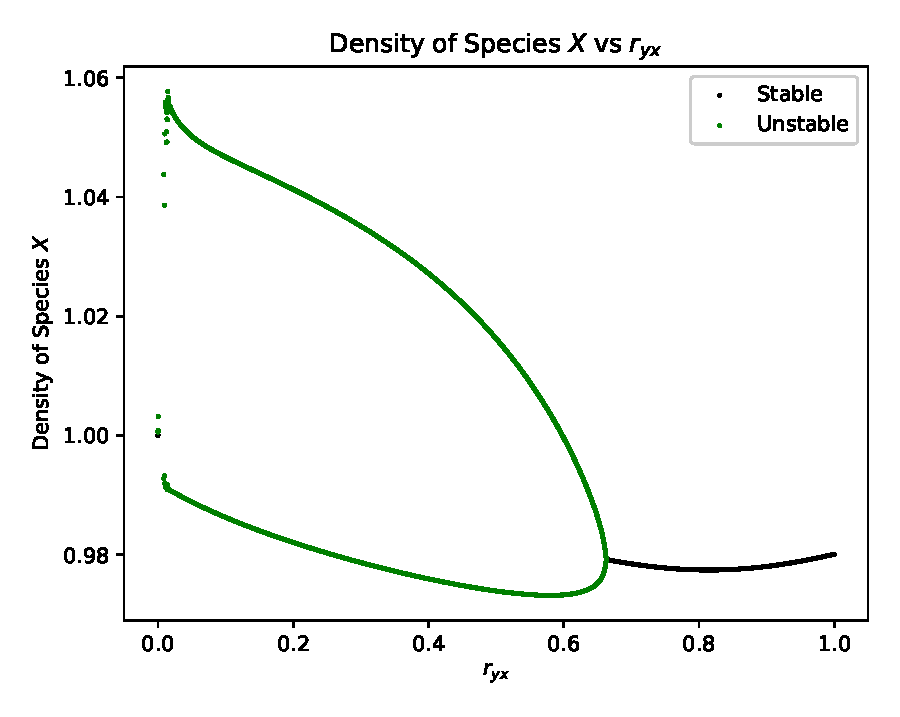
\includegraphics{equilibrium-interior-bifurcation-r_yx-x.eps}\label{fig:bifurcation-r_yx-x}}}\hspace{5pt}
    \subfloat[Bifurcation diagram of Species $Y$]{%
    \resizebox*{5cm}{!}{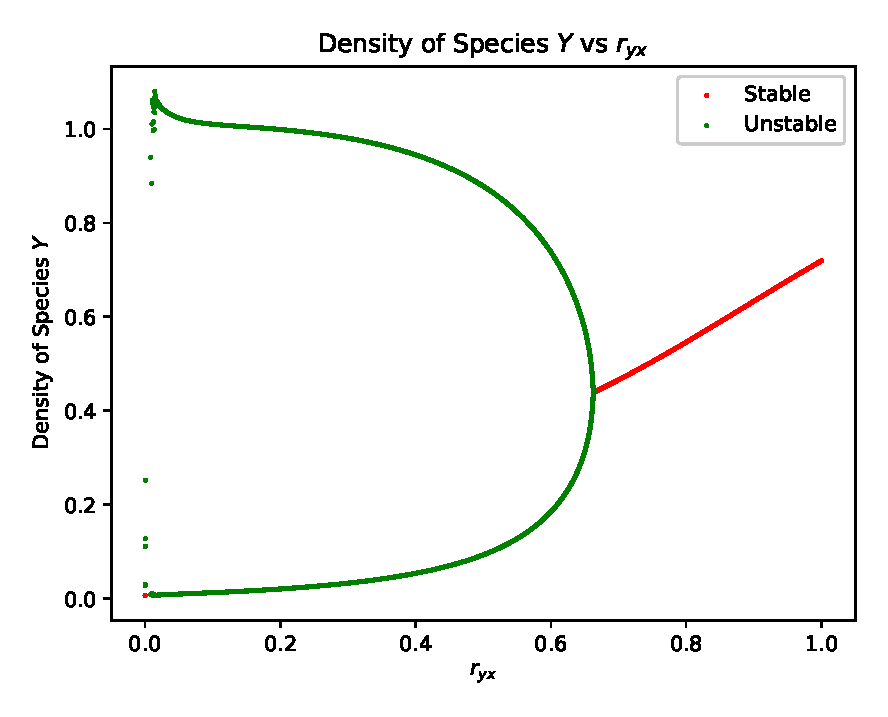
\includegraphics{equilibrium-interior-bifurcation-r_yx-y.eps}\label{fig:bifurcation-r_yx-y}}}\hspace{5pt}
    \subfloat[Bifurcation diagram of Species $Z$]{%
    \resizebox*{5cm}{!}{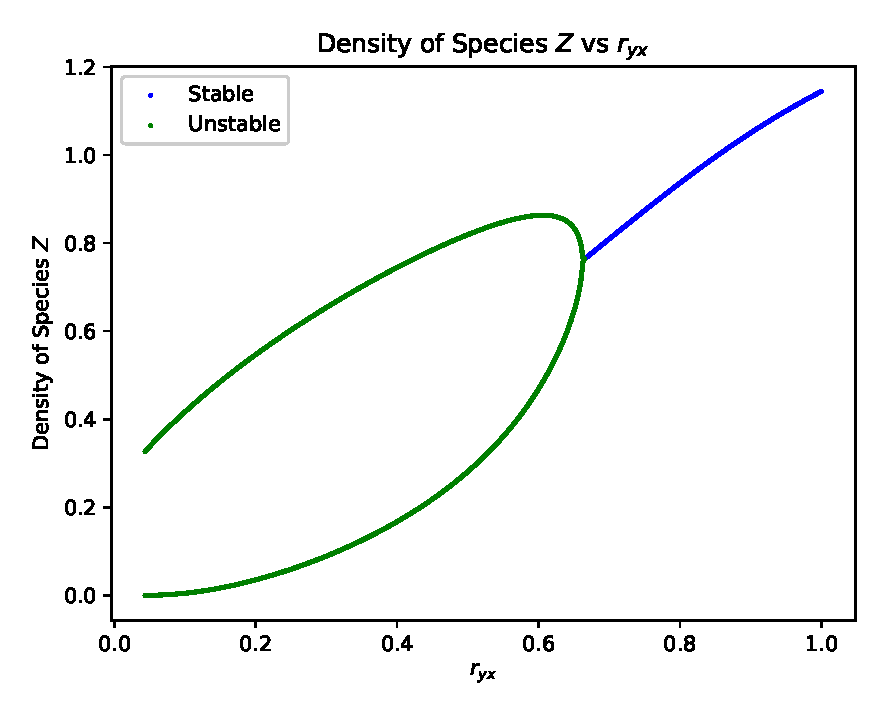
\includegraphics{equilibrium-interior-bifurcation-r_yx-z.eps}\label{fig:bifurcation-r_yx-z}}}
    \caption{Time evolution of \myref[Model]{model:rayla-ephraim} at a specific value for $r_{yx}$ under the set of \myref[parameters]{params:interior-b} and bifurcation diagrams of each species with respect to $r_{yx}$.}
    \label{fig:bifurcation-r_yx}
\end{figure}

\begin{figure}[!htb]
    \centering
    \subfloat[Time Evolution of each species where $r_{zx}=0.35$]{%
    \resizebox*{5cm}{!}{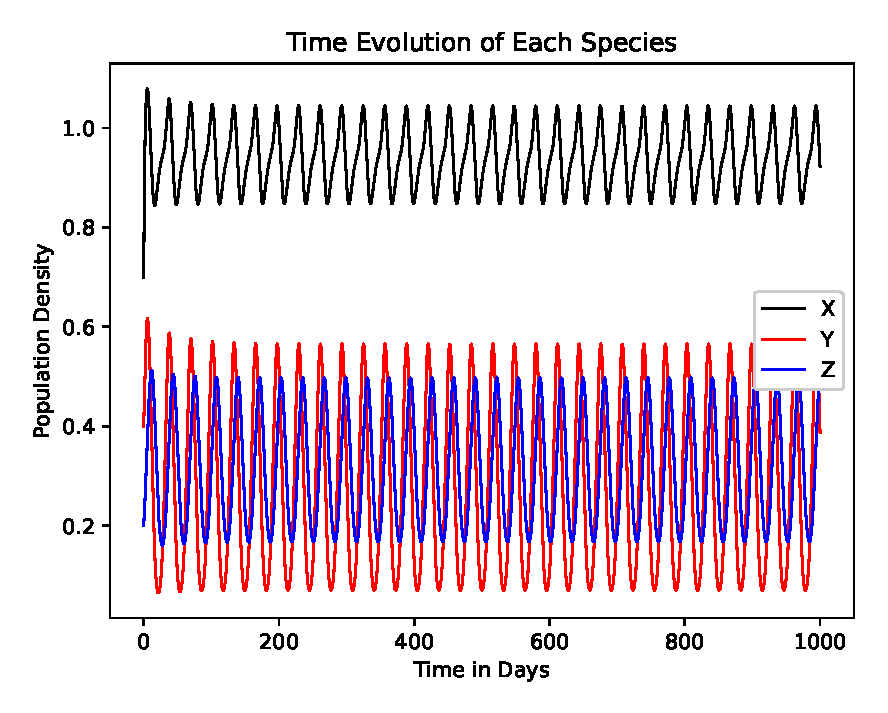
\includegraphics{equilibrium-interior-bifurcation-r_zx.eps}\label{fig:bifurcation-r_zx-xyz}}}\hspace{5pt}
    \subfloat[Bifurcation diagram of Species $X$]{%
    \resizebox*{5cm}{!}{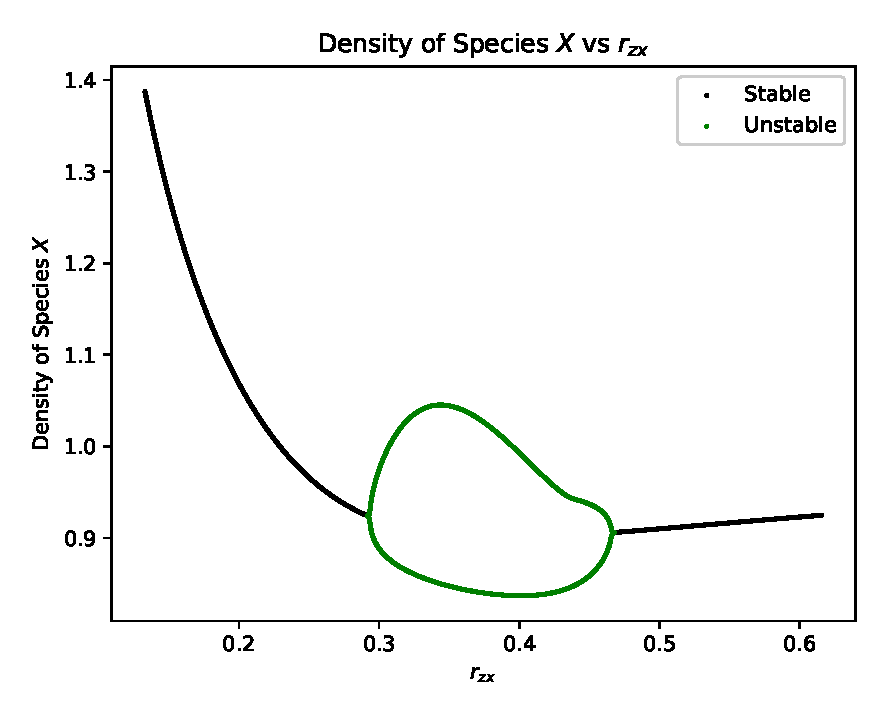
\includegraphics{equilibrium-interior-bifurcation-r_zx-x.eps}\label{fig:bifurcation-r_zx-x}}}\hspace{5pt}
    \subfloat[Bifurcation diagram of Species $Y$]{%
    \resizebox*{5cm}{!}{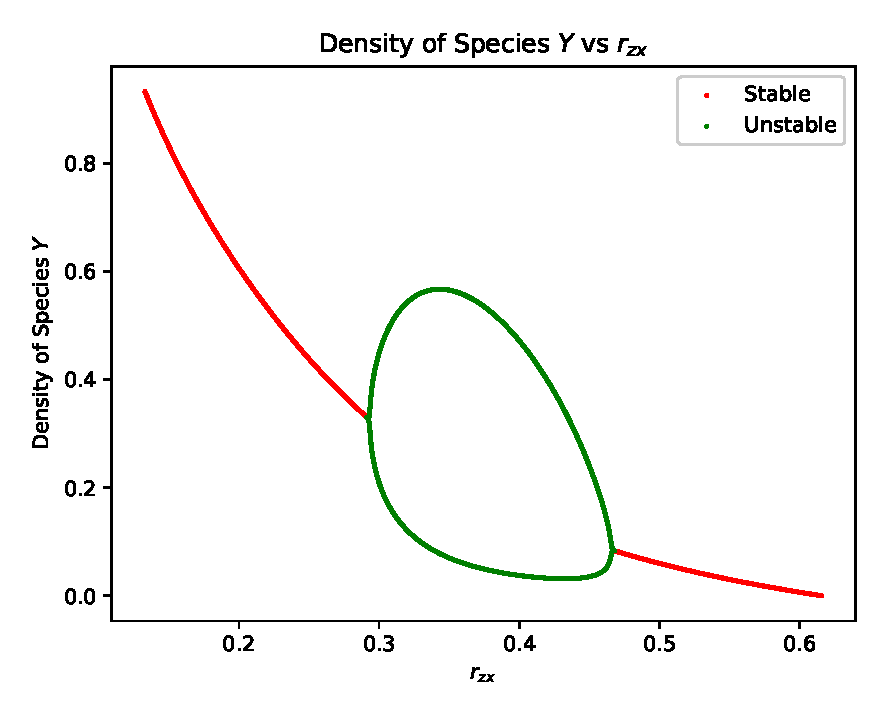
\includegraphics{equilibrium-interior-bifurcation-r_zx-y.eps}\label{fig:bifurcation-r_zx-y}}}\hspace{5pt}
    \subfloat[Bifurcation diagram of Species $Z$]{%
    \resizebox*{5cm}{!}{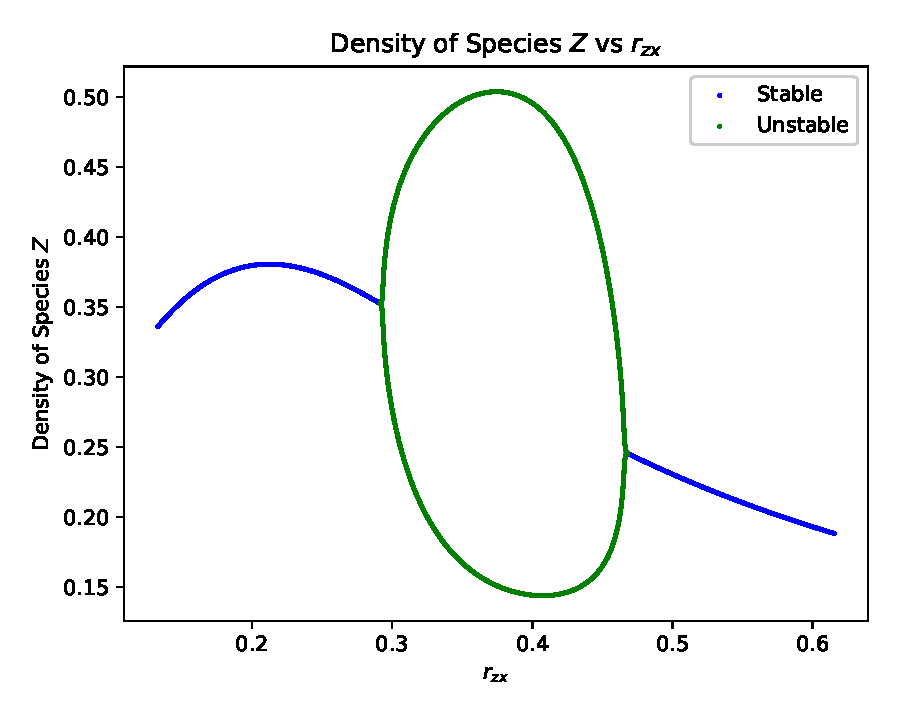
\includegraphics{equilibrium-interior-bifurcation-r_zx-z.eps}\label{fig:bifurcation-r_zx-z}}}
    \caption{Time evolution of \myref[Model]{model:rayla-ephraim} at a specific value for $r_{zx}$ under the set of \myref[parameters]{params:interior-a} and bifurcation diagrams of each species with respect to $r_{zx}$.}
    \label{fig:bifurcation-r_zx}
\end{figure}

\begin{figure}[!htb]
    \centering
    \subfloat[Time Evolution of each species where $p=0.1$]{%
    \resizebox*{5cm}{!}{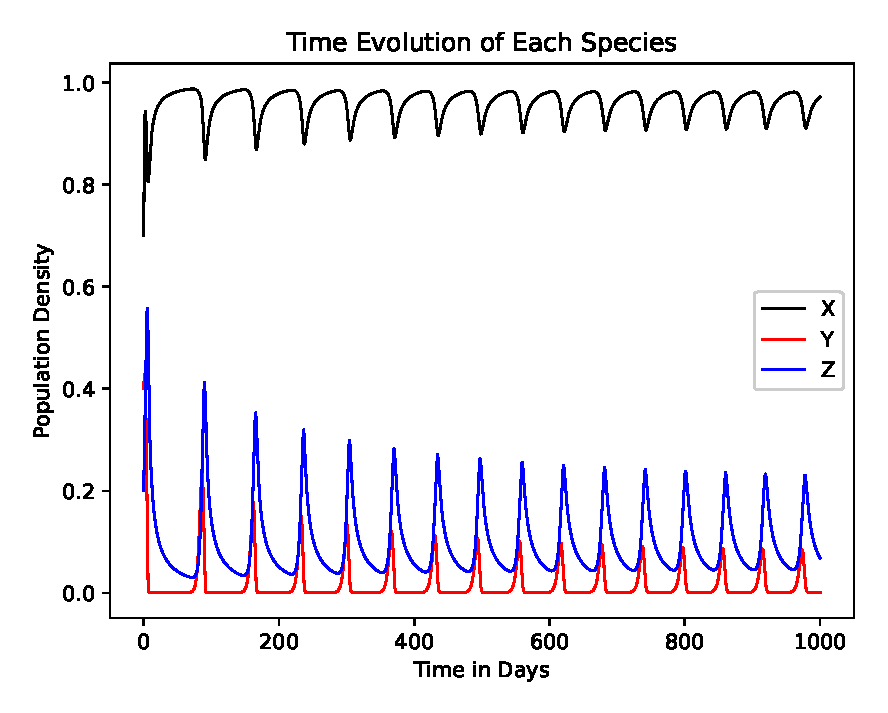
\includegraphics{equilibrium-interior-bifurcation-p.eps}\label{fig:bifurcation-p-xyz}}}\hspace{5pt}
    \subfloat[Bifurcation diagram of Species $X$]{%
    \resizebox*{5cm}{!}{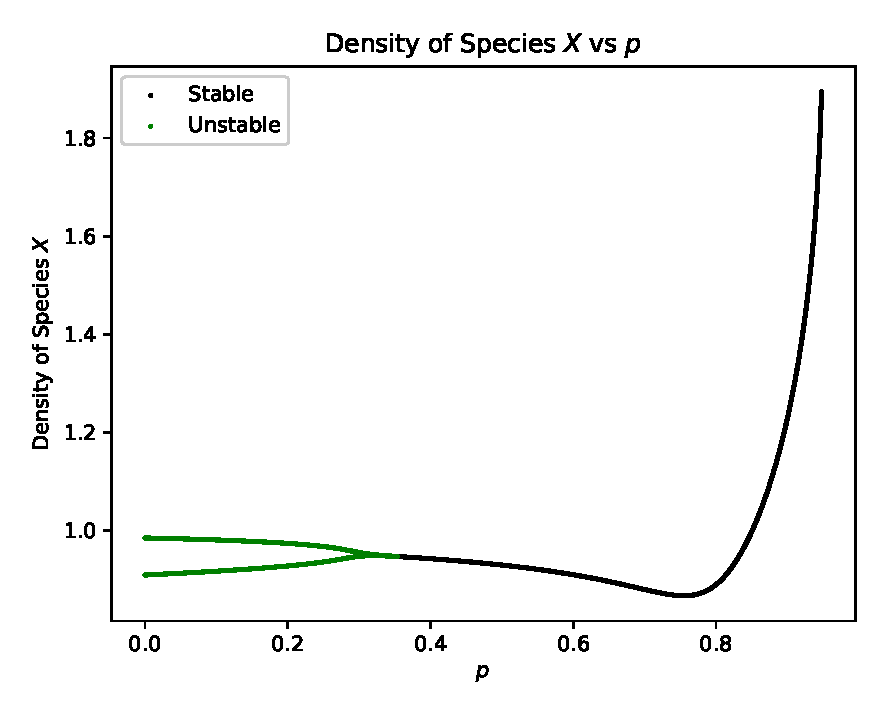
\includegraphics{equilibrium-interior-bifurcation-p-x.eps}\label{fig:bifurcation-p-x}}}\hspace{5pt}
    \subfloat[Bifurcation diagram of Species $Y$]{%
    \resizebox*{5cm}{!}{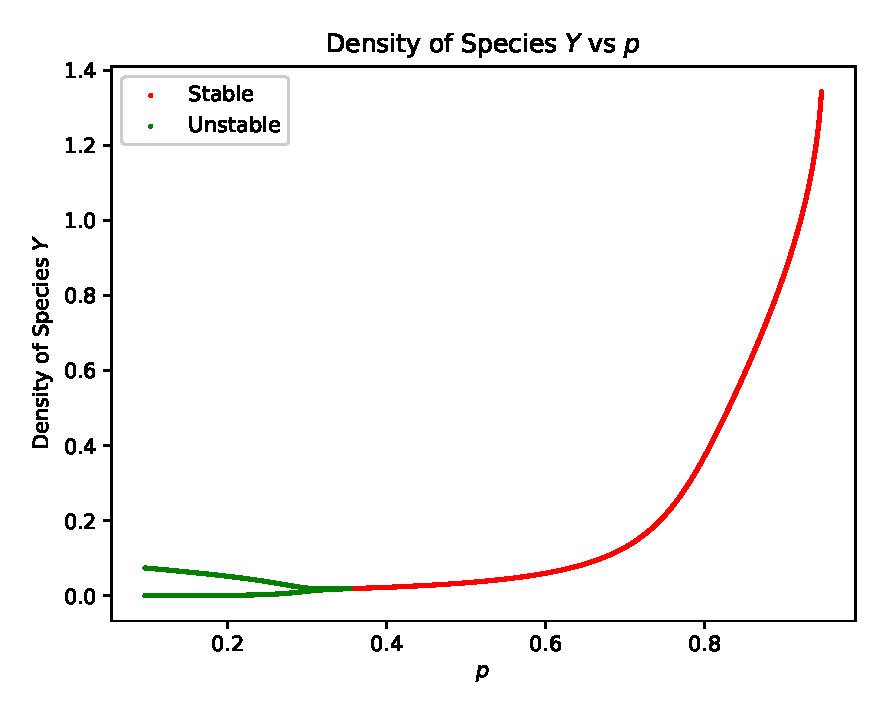
\includegraphics{equilibrium-interior-bifurcation-p-y.eps}\label{fig:bifurcation-p-y}}}\hspace{5pt}
    \subfloat[Bifurcation diagram of Species $Z$]{%
    \resizebox*{5cm}{!}{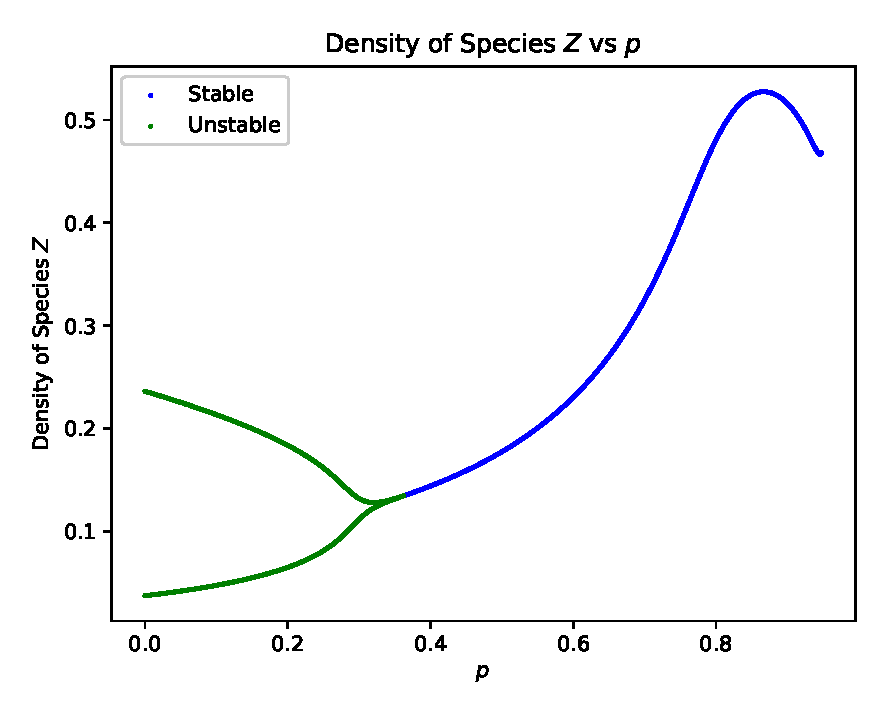
\includegraphics{equilibrium-interior-bifurcation-p-z.eps}\label{fig:bifurcation-p-z}}}
    \caption{Time evolution of \myref[Model]{model:rayla-ephraim} at a specific value for $p$ under the set of \myref[parameters]{params:interior-a} and bifurcation diagrams of each species with respect to $p$.}
    \label{fig:bifurcation-p}
\end{figure}

\begin{figure}[!htb]
    \centering
    \subfloat[Time Evolution of each species where $\varphi_{xy}=0.15$]{%
    \resizebox*{5cm}{!}{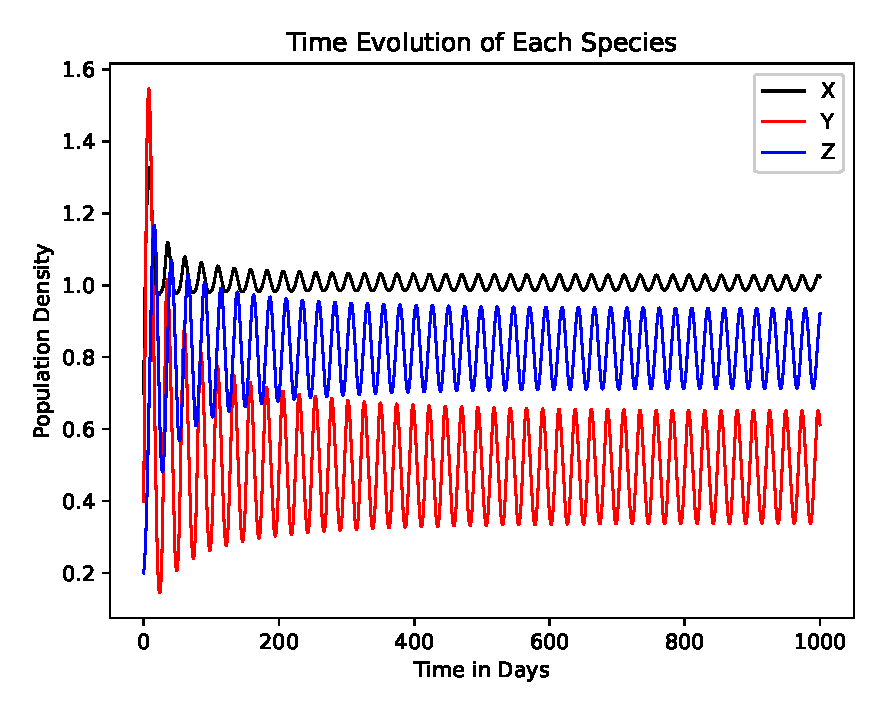
\includegraphics{equilibrium-interior-bifurcation-phi_xy.eps}\label{fig:bifurcation-phi_xy-xyz}}}\hspace{5pt}
    \subfloat[Bifurcation diagram of Species $X$]{%
    \resizebox*{5cm}{!}{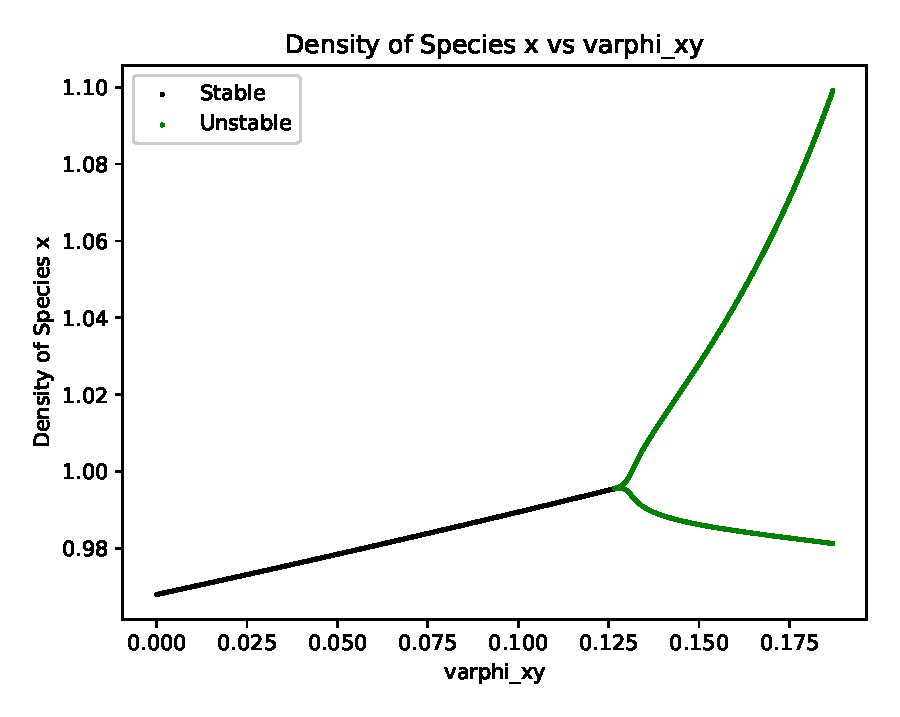
\includegraphics{equilibrium-interior-bifurcation-phi_xy-x.eps}\label{fig:bifurcation-phi_xy-x}}}\hspace{5pt}
    \subfloat[Bifurcation diagram of Species $Y$]{%
    \resizebox*{5cm}{!}{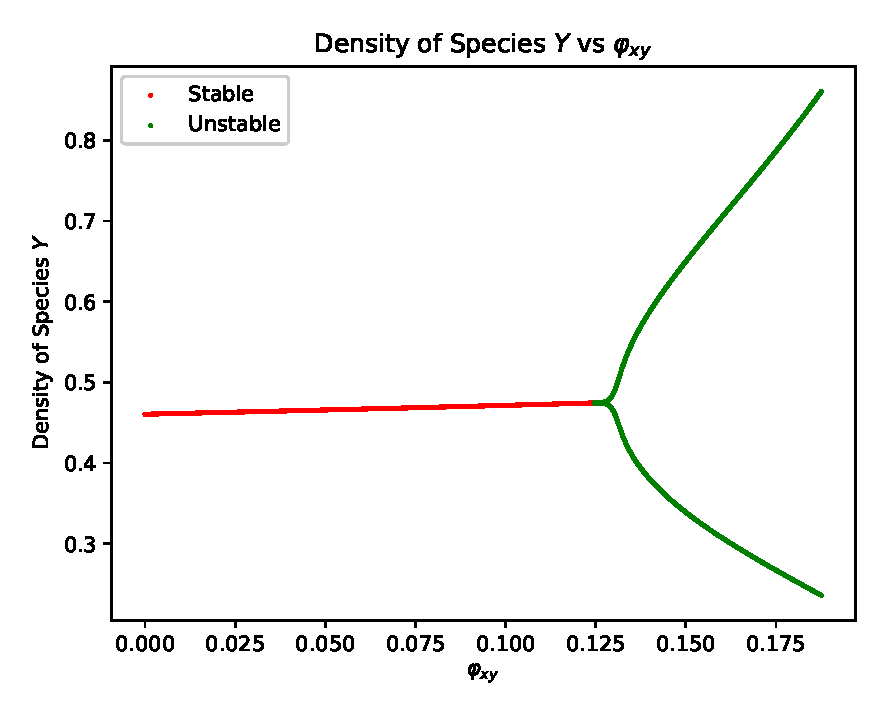
\includegraphics{equilibrium-interior-bifurcation-phi_xy-y.eps}\label{fig:bifurcation-phi_xy-y}}}\hspace{5pt}
    \subfloat[Bifurcation diagram of Species $Z$]{%
    \resizebox*{5cm}{!}{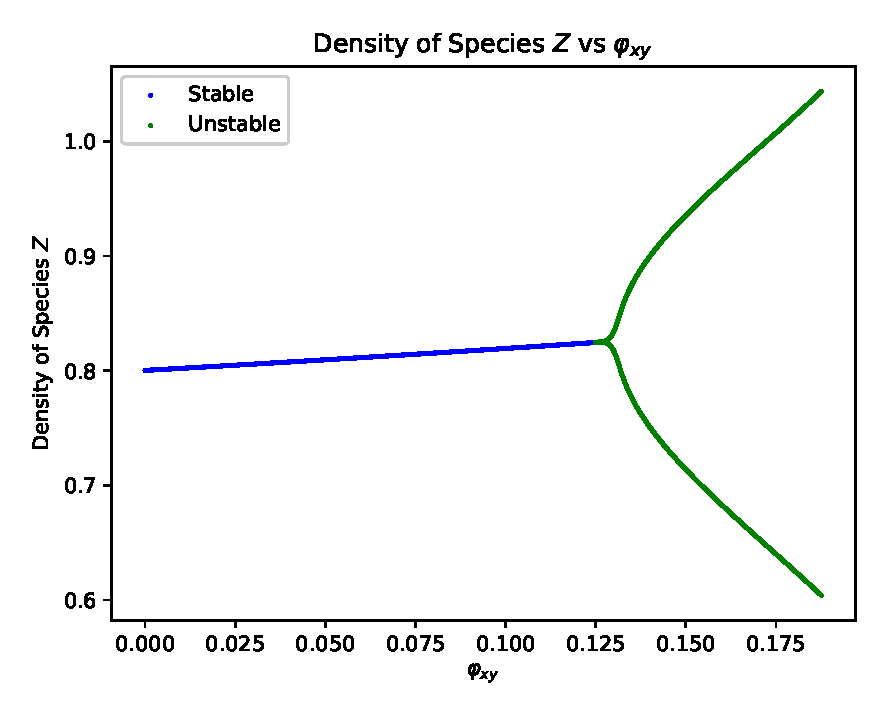
\includegraphics{equilibrium-interior-bifurcation-phi_xy-z.eps}\label{fig:bifurcation-phi_xy-z}}}
    \caption{Time evolution of \myref[Model]{model:rayla-ephraim} at a specific value for $\varphi_{xy}$ under the set of \myref[parameters]{params:interior-b} and bifurcation diagrams of each species with respect to $\varphi_{xy}$.}
    \label{fig:bifurcation-phi_xy}
\end{figure}

\begin{figure}[!htb]
    \centering
    \subfloat[Time Evolution of each species where $\varphi_{yx}=0.43$]{%
    \resizebox*{5cm}{!}{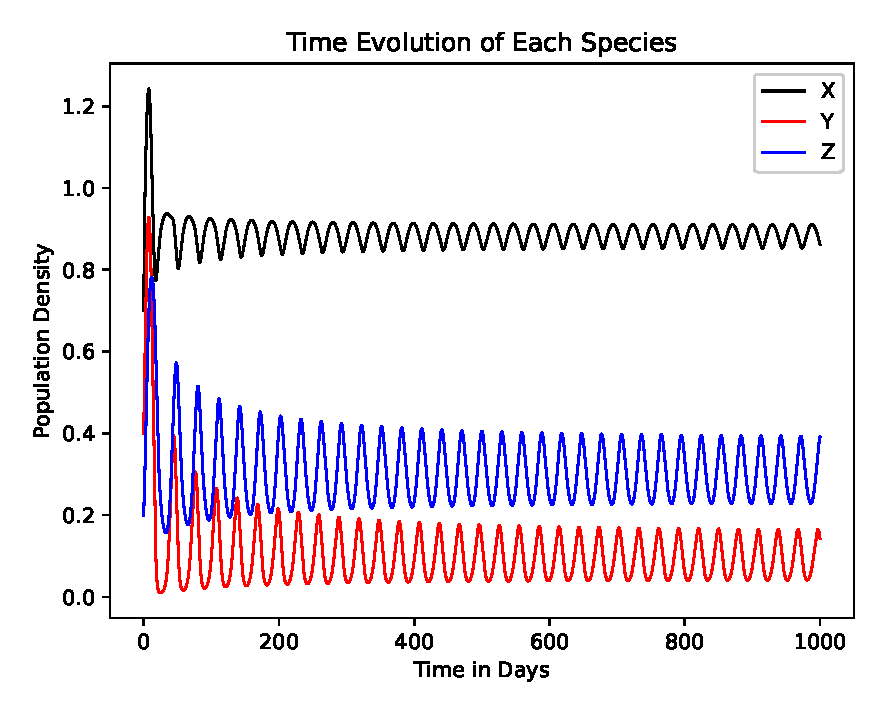
\includegraphics{equilibrium-interior-bifurcation-phi_yx.eps}\label{fig:bifurcation-phi_yx-xyz}}}\hspace{5pt}
    \subfloat[Bifurcation diagram of Species $X$]{%
    \resizebox*{5cm}{!}{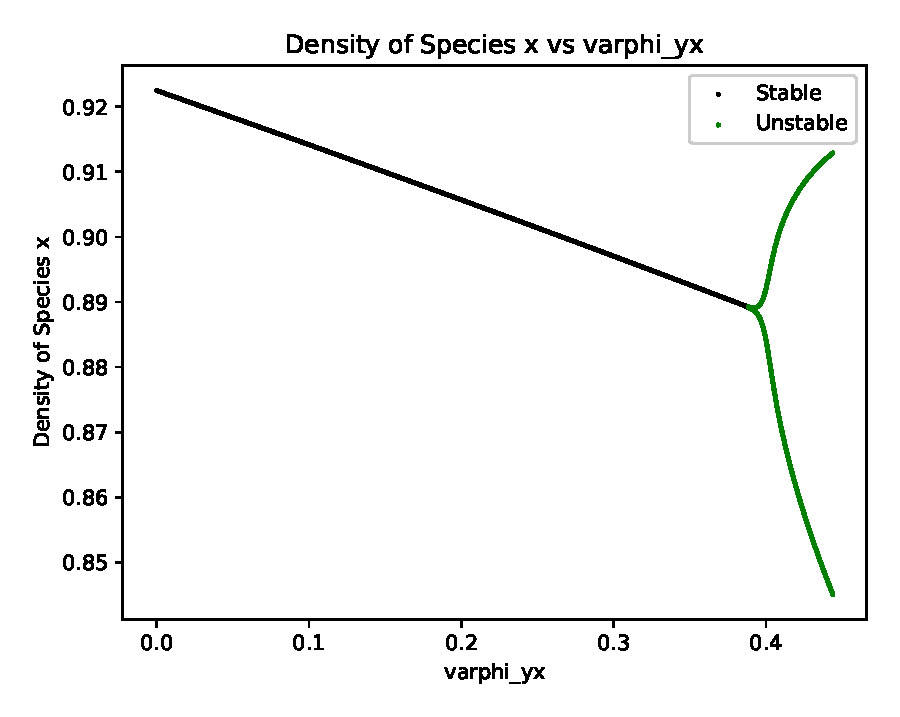
\includegraphics{equilibrium-interior-bifurcation-phi_yx-x.eps}\label{fig:bifurcation-phi_yx-x}}}\hspace{5pt}
    \subfloat[Bifurcation diagram of Species $Y$]{%
    \resizebox*{5cm}{!}{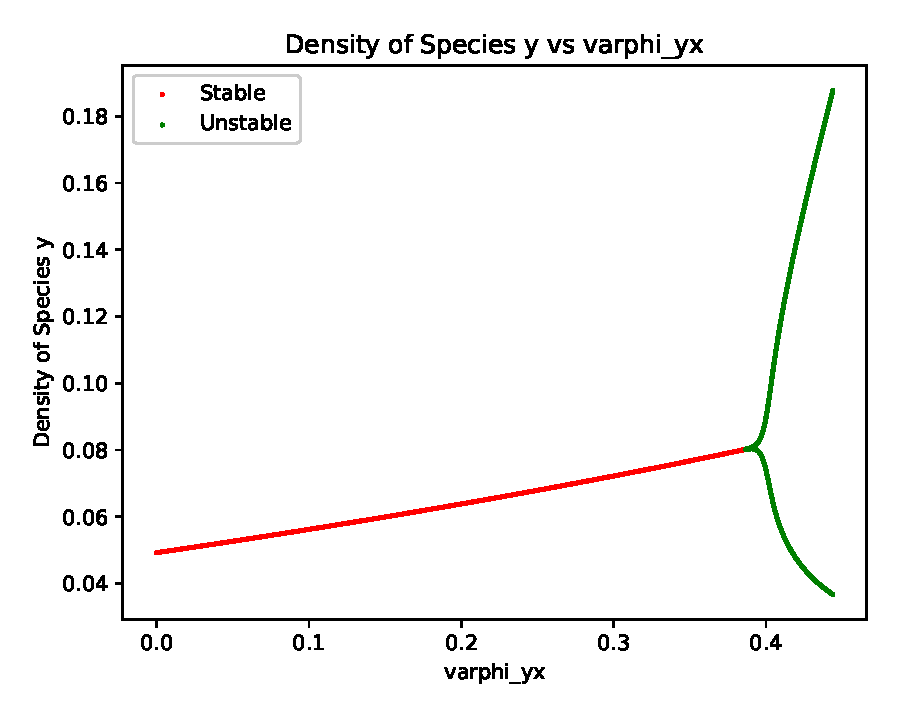
\includegraphics{equilibrium-interior-bifurcation-phi_yx-y.eps}\label{fig:bifurcation-phi_yx-y}}}\hspace{5pt}
    \subfloat[Bifurcation diagram of Species $Z$]{%
    \resizebox*{5cm}{!}{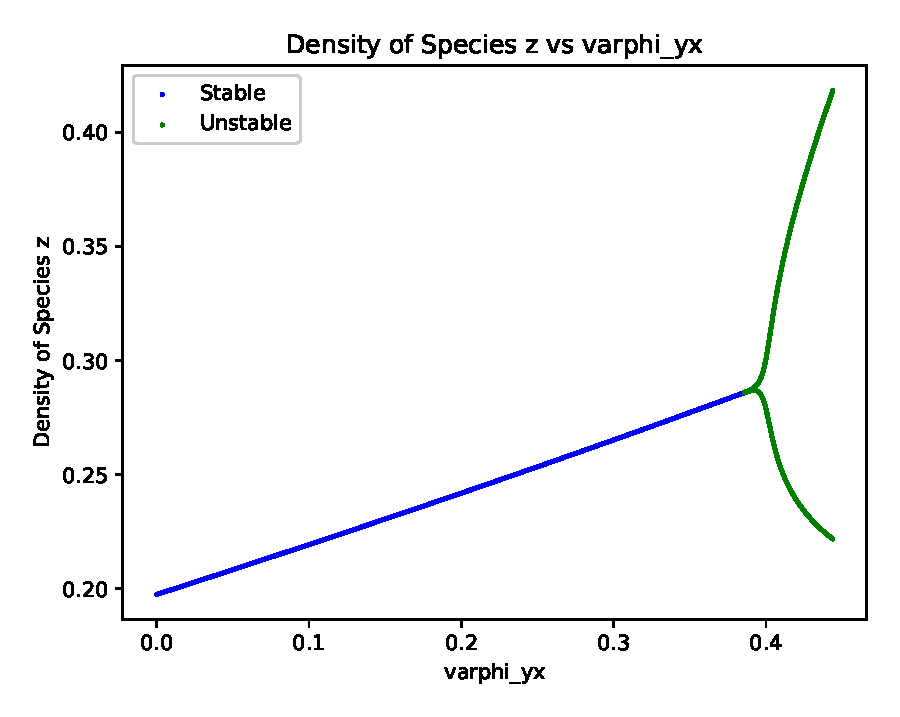
\includegraphics{equilibrium-interior-bifurcation-phi_yx-z.eps}\label{fig:bifurcation-phi_yx-z}}}
    \caption{Time evolution of \myref[Model]{model:rayla-ephraim} at a specific value for $\varphi_{yx}$ under the set of \myref[parameters]{params:interior-a} and bifurcation diagrams of each species with respect to $\varphi_{yx}$.}
    \label{fig:bifurcation-phi_yx}
\end{figure}

\begin{figure}[!htb]
    \centering
    \subfloat[Time Evolution of each species where $\varphi_{xz}=0.5$]{%
    \resizebox*{5cm}{!}{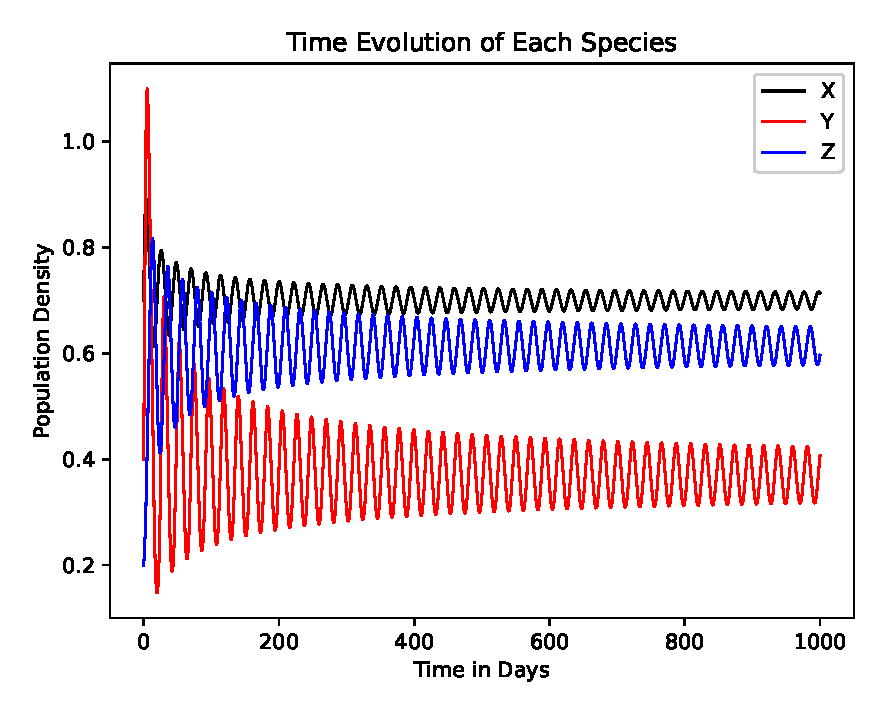
\includegraphics{equilibrium-interior-bifurcation-phi_xz.eps}\label{fig:bifurcation-phi_xz-xyz}}}\hspace{5pt}
    \subfloat[Bifurcation diagram of Species $X$]{%
    \resizebox*{5cm}{!}{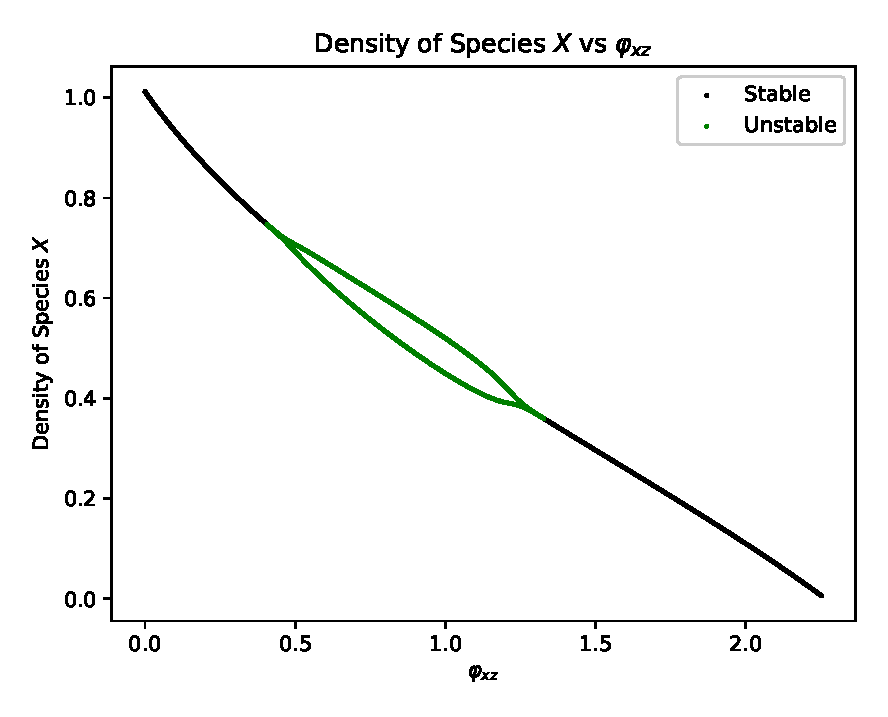
\includegraphics{equilibrium-interior-bifurcation-phi_xz-x.eps}\label{fig:bifurcation-phi_xz-x}}}\hspace{5pt}
    \subfloat[Bifurcation diagram of Species $Y$]{%
    \resizebox*{5cm}{!}{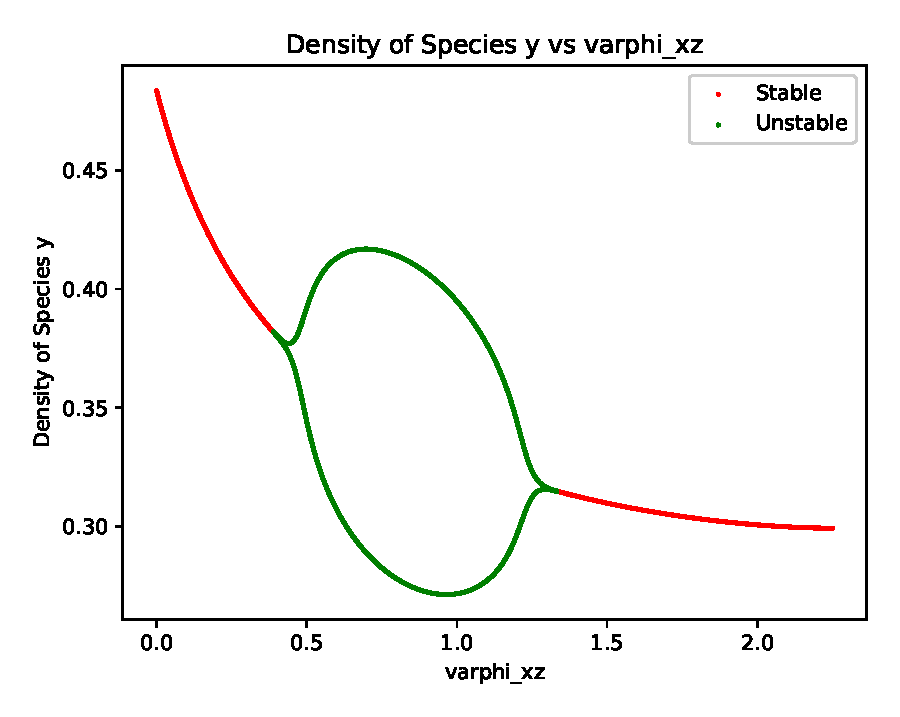
\includegraphics{equilibrium-interior-bifurcation-phi_xz-y.eps}\label{fig:bifurcation-phi_xz-y}}}\hspace{5pt}
    \subfloat[Bifurcation diagram of Species $Z$]{%
    \resizebox*{5cm}{!}{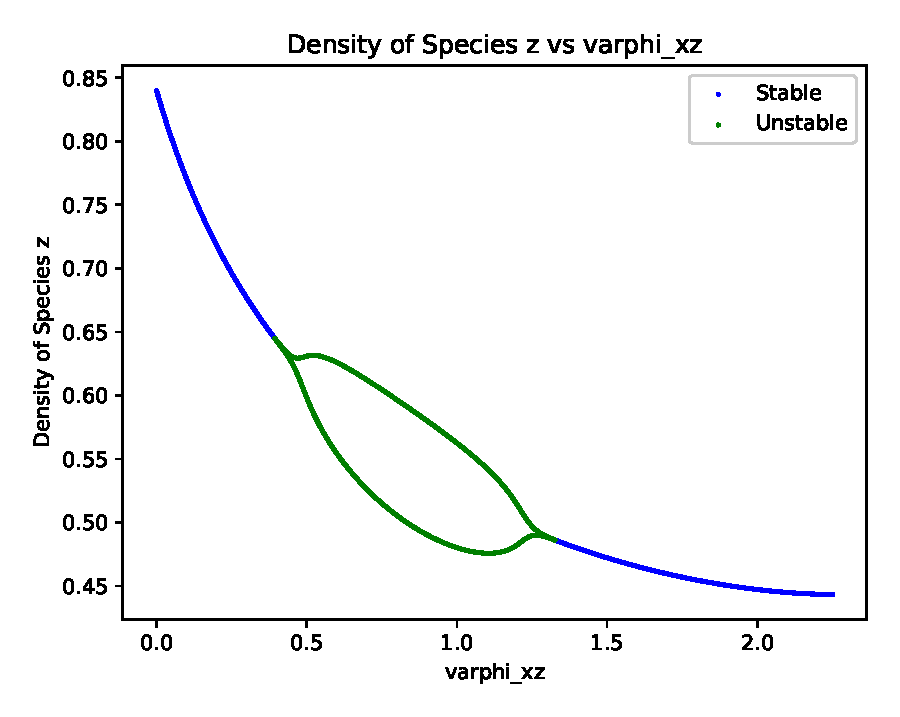
\includegraphics{equilibrium-interior-bifurcation-phi_xz-z.eps}\label{fig:bifurcation-phi_xz-z}}}
    \caption{Time evolution of \myref[Model]{model:rayla-ephraim} at a specific value for $\varphi_{xz}$ under the set of \myref[parameters]{params:interior-b} and bifurcation diagrams of each species with respect to $\varphi_{xz}$.}
    \label{fig:bifurcation-phi_xz}
\end{figure}

\begin{figure}[!htb]
    \centering
    \subfloat[Time Evolution of each species where $u_1=0.8$]{%
    \resizebox*{5cm}{!}{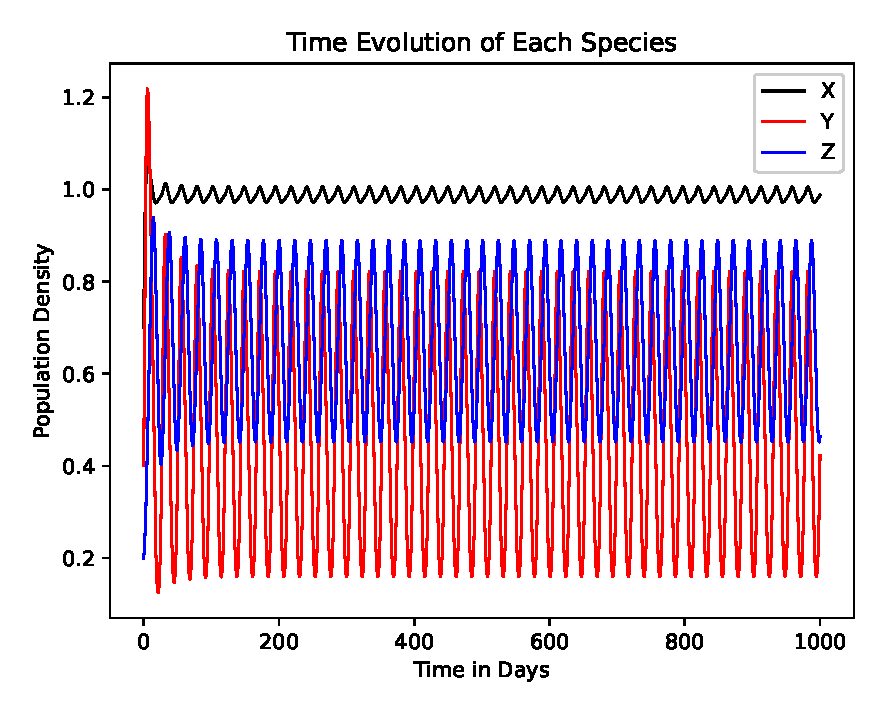
\includegraphics{equilibrium-interior-bifurcation-u_1.eps}\label{fig:bifurcation-u_1-xyz}}}\hspace{5pt}
    \subfloat[Bifurcation diagram of Species $X$]{%
    \resizebox*{5cm}{!}{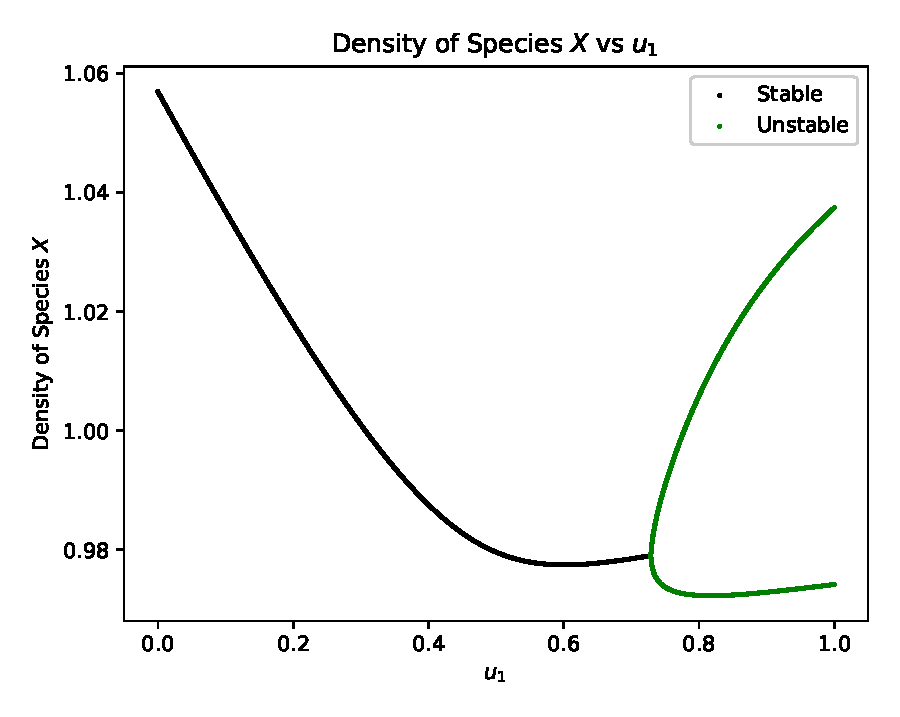
\includegraphics{equilibrium-interior-bifurcation-u_1-x.eps}\label{fig:bifurcation-u_1-x}}}\hspace{5pt}
    \subfloat[Bifurcation diagram of Species $Y$]{%
    \resizebox*{5cm}{!}{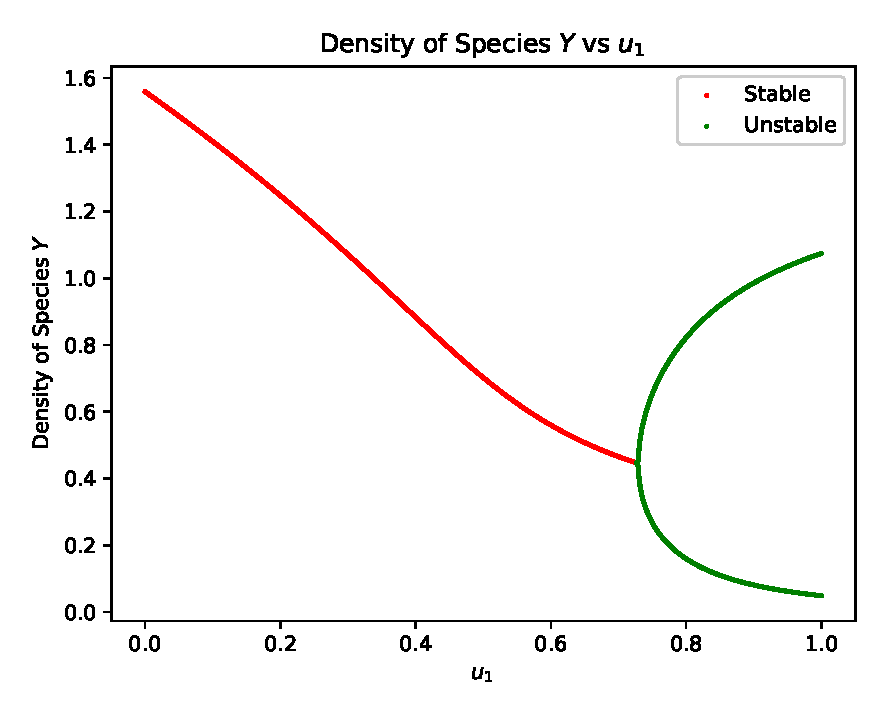
\includegraphics{equilibrium-interior-bifurcation-u_1-y.eps}\label{fig:bifurcation-u_1-y}}}\hspace{5pt}
    \subfloat[Bifurcation diagram of Species $Z$]{%
    \resizebox*{5cm}{!}{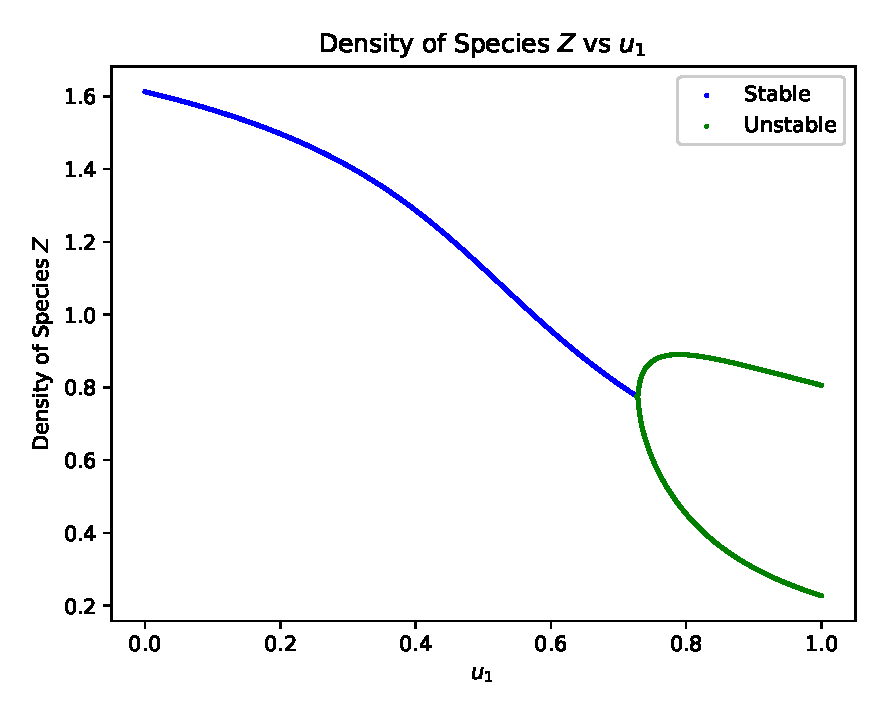
\includegraphics{equilibrium-interior-bifurcation-u_1-z.eps}\label{fig:bifurcation-u_1-z}}}
    \caption{Time evolution of \myref[Model]{model:rayla-ephraim} at a specific value for $u_1$ under the set of \myref[parameters]{params:interior-b} and bifurcation diagrams of each species with respect to $u_1$.}
    \label{fig:bifurcation-u_1}
\end{figure}

\begin{figure}[!htb]
    \centering
    \subfloat[Time Evolution of each species where $u_2=0.04$]{%
    \resizebox*{5cm}{!}{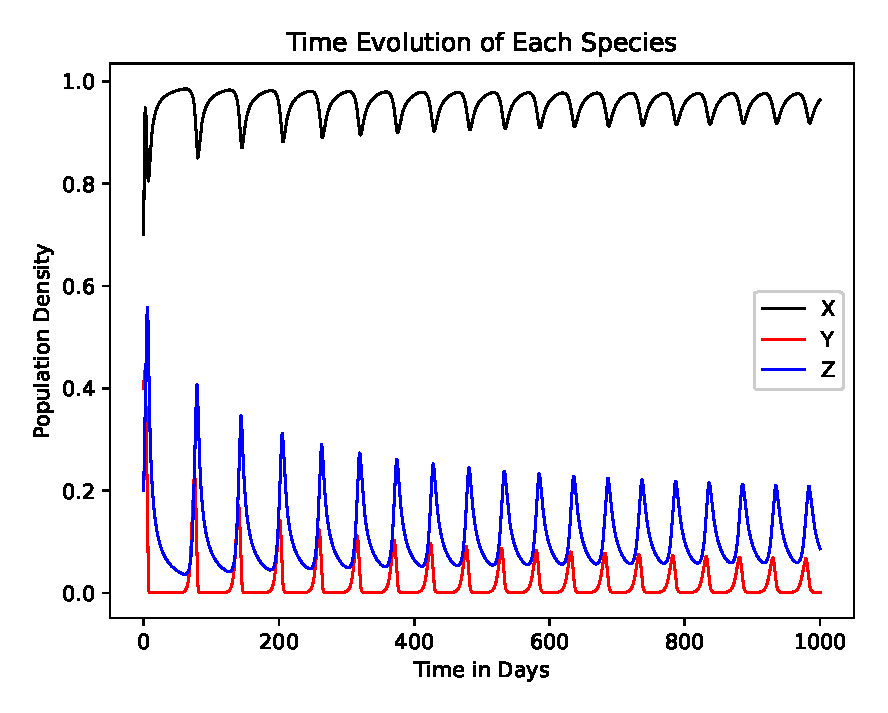
\includegraphics{equilibrium-interior-bifurcation-u_2.eps}\label{fig:bifurcation-u_2-xyz}}}\hspace{5pt}
    \subfloat[Bifurcation diagram of Species $X$]{%
    \resizebox*{5cm}{!}{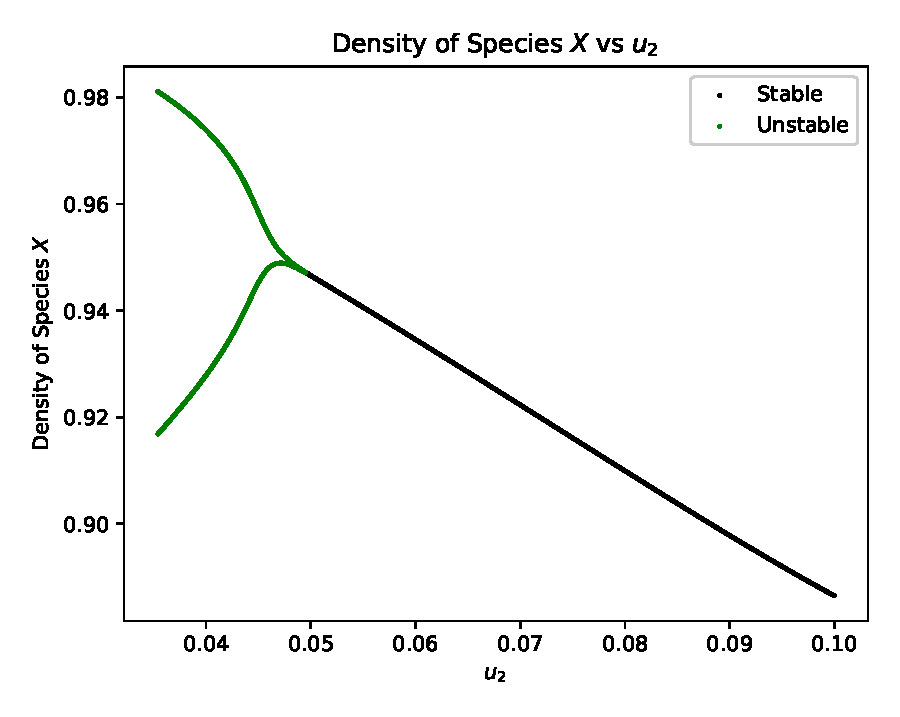
\includegraphics{equilibrium-interior-bifurcation-u_2-x.eps}\label{fig:bifurcation-u_2-x}}}\hspace{5pt}
    \subfloat[Bifurcation diagram of Species $Y$]{%
    \resizebox*{5cm}{!}{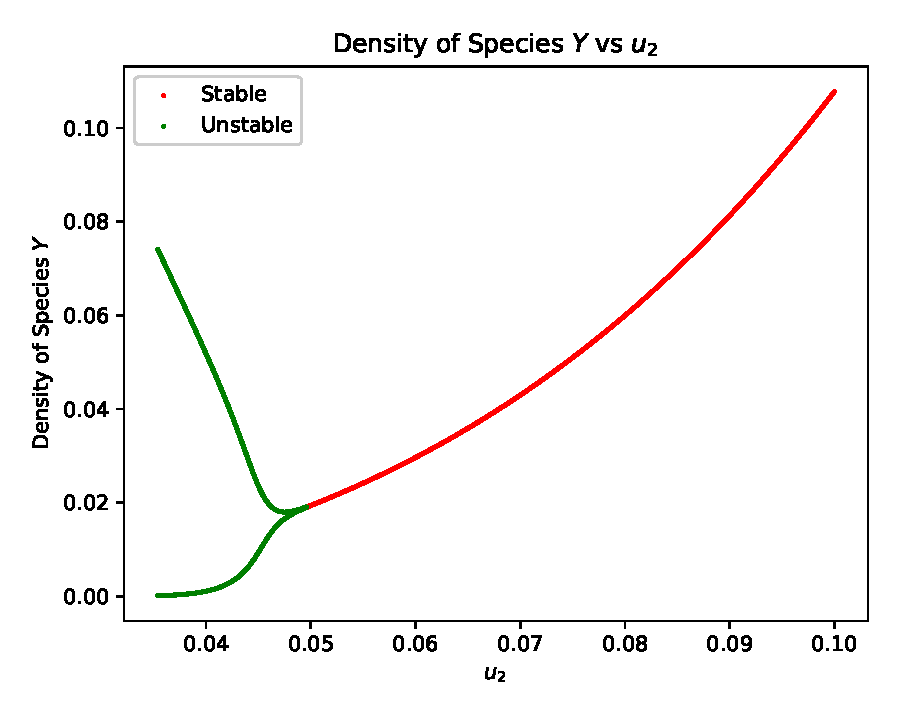
\includegraphics{equilibrium-interior-bifurcation-u_2-y.eps}\label{fig:bifurcation-u_2-y}}}\hspace{5pt}
    \subfloat[Bifurcation diagram of Species $Z$]{%
    \resizebox*{5cm}{!}{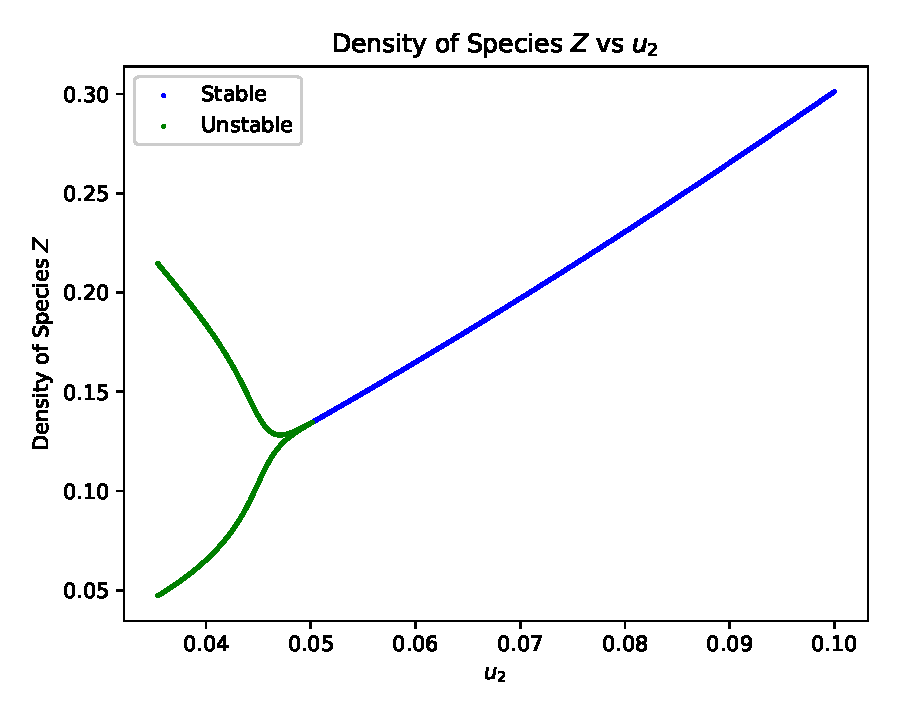
\includegraphics{equilibrium-interior-bifurcation-u_2-z.eps}\label{fig:bifurcation-u_2-z}}}
    \caption{Time evolution of \myref[Model]{model:rayla-ephraim} at a specific value for $u_2$ under the set of \myref[parameters]{params:interior-a} and bifurcation diagrams of each species with respect to $u_2$.}
    \label{fig:bifurcation-u_2}
\end{figure}

\begin{figure}[!htb]
    \centering
    \subfloat[Time Evolution of each species where $u_3=0.75$]{%
    \resizebox*{5cm}{!}{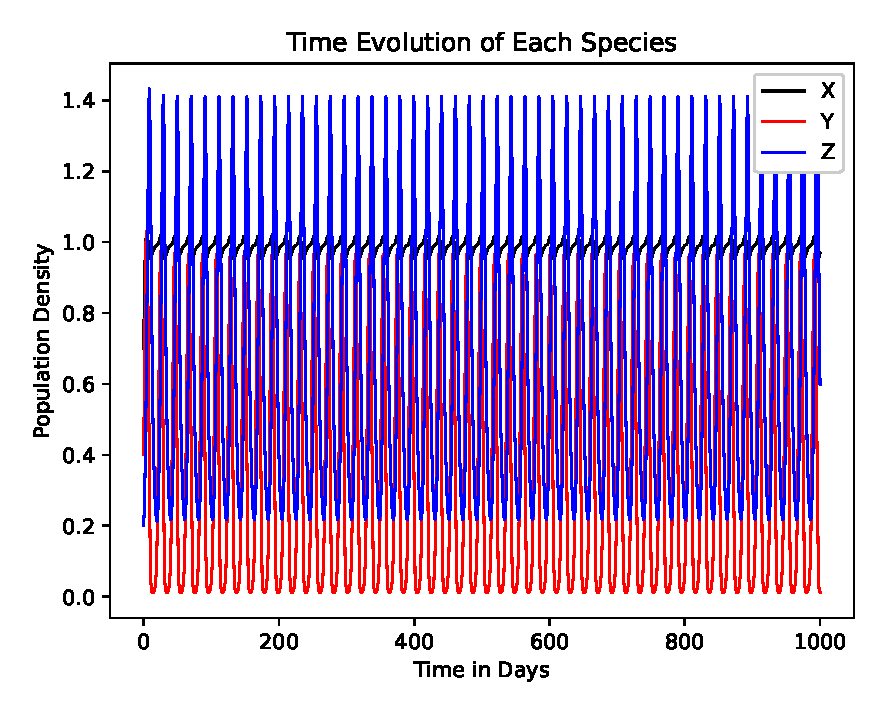
\includegraphics{equilibrium-interior-bifurcation-u_3.eps}\label{fig:bifurcation-u_3-xyz}}}\hspace{5pt}
    \subfloat[Bifurcation diagram of Species $X$]{%
    \resizebox*{5cm}{!}{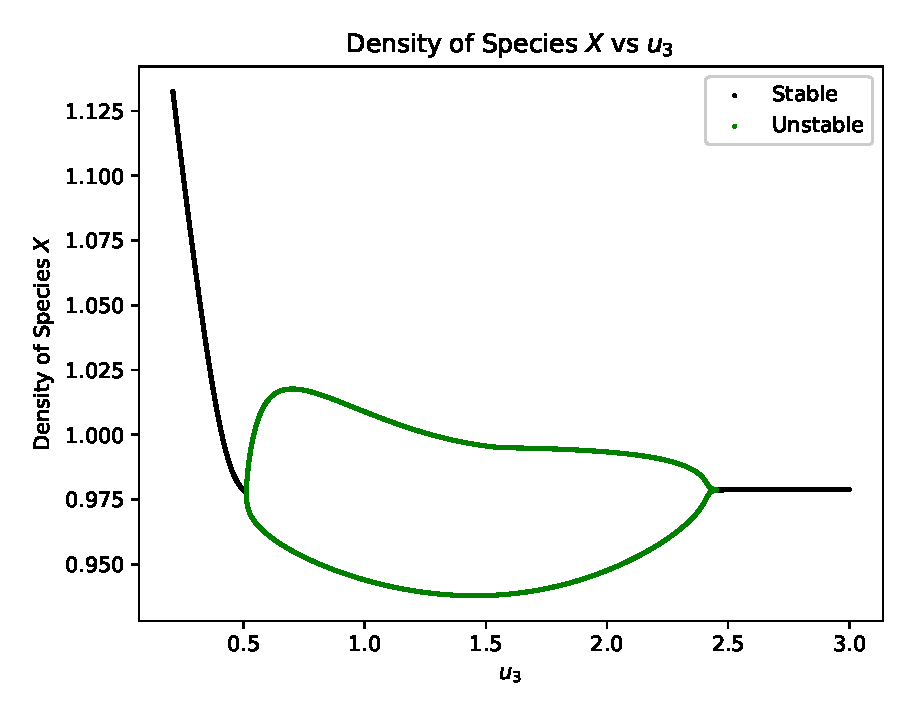
\includegraphics{equilibrium-interior-bifurcation-u_3-x.eps}\label{fig:bifurcation-u_3-x}}}\hspace{5pt}
    \subfloat[Bifurcation diagram of Species $Y$]{%
    \resizebox*{5cm}{!}{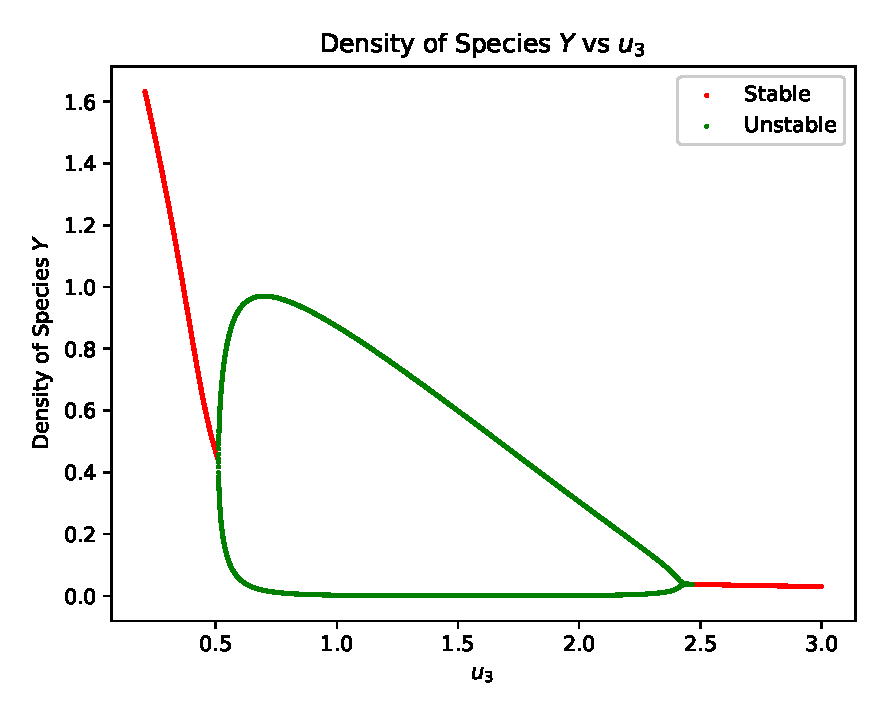
\includegraphics{equilibrium-interior-bifurcation-u_3-y.eps}\label{fig:bifurcation-u_3-y}}}\hspace{5pt}
    \subfloat[Bifurcation diagram of Species $Z$]{%
    \resizebox*{5cm}{!}{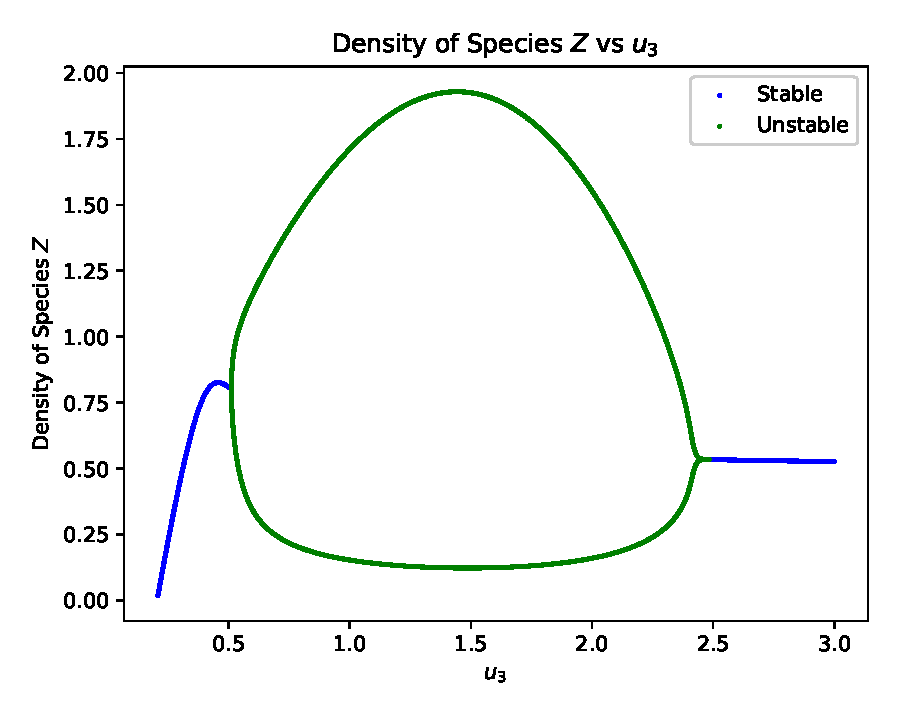
\includegraphics{equilibrium-interior-bifurcation-u_3-z.eps}\label{fig:bifurcation-u_3-z}}}
    \caption{Time evolution of \myref[Model]{model:rayla-ephraim} at a specific value for $u_3$ under the set of \myref[parameters]{params:interior-b} and bifurcation diagrams of each species with respect to $u_3$.}
    \label{fig:bifurcation-u_3}
\end{figure}

\begin{figure}[!htb]
    \centering
    \subfloat[Time Evolution of each species where $u_4=0.3$]{%
    \resizebox*{5cm}{!}{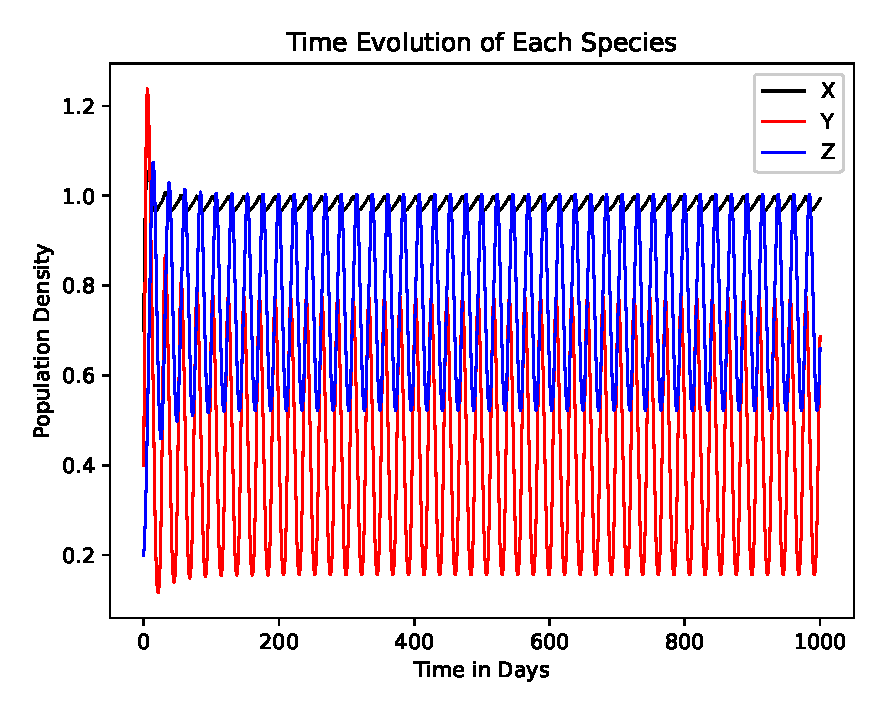
\includegraphics{equilibrium-interior-bifurcation-u_4.eps}\label{fig:bifurcation-u_4-xyz}}}\hspace{5pt}
    \subfloat[Bifurcation diagram of Species $X$]{%
    \resizebox*{5cm}{!}{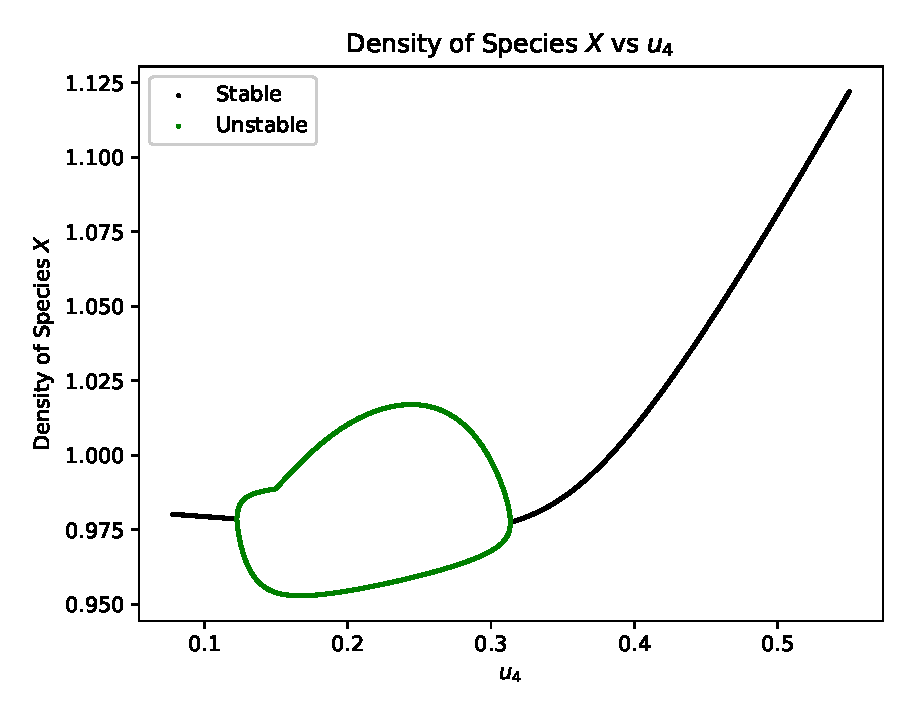
\includegraphics{equilibrium-interior-bifurcation-u_4-x.eps}\label{fig:bifurcation-u_4-x}}}\hspace{5pt}
    \subfloat[Bifurcation diagram of Species $Y$]{%
    \resizebox*{5cm}{!}{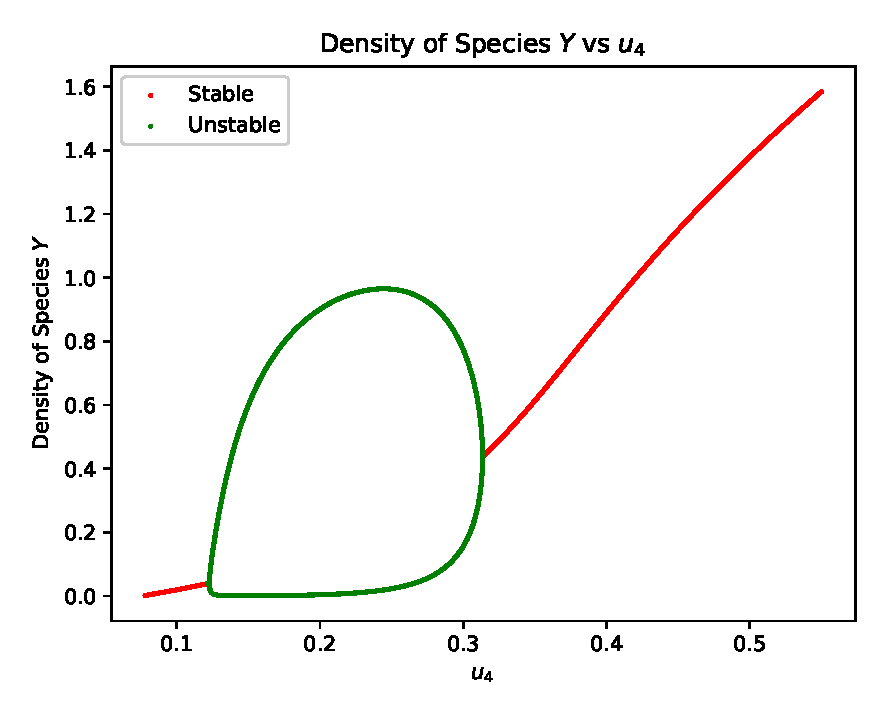
\includegraphics{equilibrium-interior-bifurcation-u_4-y.eps}\label{fig:bifurcation-u_4-y}}}\hspace{5pt}
    \subfloat[Bifurcation diagram of Species $Z$]{%
    \resizebox*{5cm}{!}{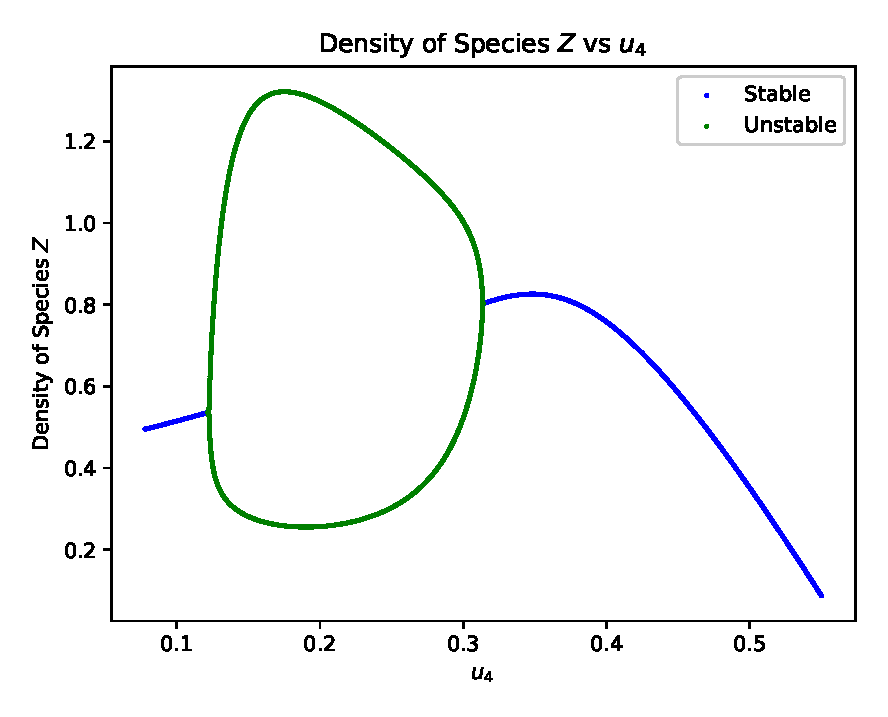
\includegraphics{equilibrium-interior-bifurcation-u_4-z.eps}\label{fig:bifurcation-u_4-z}}}
    \caption{Time evolution of \myref[Model]{model:rayla-ephraim} at a specific value for $u_4$ under the set of \myref[parameters]{params:interior-b} and bifurcation diagrams of each species with respect to $u_4$.}
    \label{fig:bifurcation-u_4}
\end{figure}
